\documentclass[a4paper]{article}
\usepackage{cmap}
\usepackage[utf8]{inputenc}
\usepackage[T2A]{fontenc}
\usepackage[english,russian]{babel} 
\usepackage[left=15mm, top=15mm, right=15mm, bottom=42mm, nohead, nofoot]{geometry}
\usepackage{blindtext}  % рыба-текст
\usepackage{graphicx}  % изобржаения
\usepackage{float} % плавающие объекты
\usepackage{wrapfig}  % изобржаения
\usepackage{tikz} % графика
\usepackage{xcolor} % определение цветов
\usepackage{nicefrac} % красивые дроби
\usepackage{cancel} % сокращение
\usepackage{amsmath,amsfonts,amssymb} % математический пакет
\usepackage{hyperref}  % гиперссылки
\usepackage{fancybox,fancyhdr} % хедер и футер
\pagestyle{fancy}
\fancyhf{}
\fancyhead[L]{Математический анализ}
\fancyhead[R]{Вариант №6}
\fancyfoot[C]{\thepage}
\setlength{\headheight}{12.0pt}
\headsep=5mm
\footskip=10mm

\definecolor{urlcolor}{HTML}{3454D1}
\definecolor{linkcolor}{HTML}{3454D1}
\hypersetup{pdfstartview=FitH, linkcolor=linkcolor, urlcolor=urlcolor, colorlinks=true}

\addto\captionsrussian{
  \renewcommand{\contentsname}
    {\centering Содержание}
}
\newcommand{\addsection}[1]{
    \phantomsection
    \addcontentsline{toc}{section}{#1}
    \section*{\centering #1}
}
\newcommand{\addsubsection}[1]{
    \phantomsection
    \addcontentsline{toc}{subsection}{#1}
    \subsection*{\centering #1}
}

\newlength{\tempheight}
\newcommand{\Let}{
\mathbin{\text{\settoheight{\tempheight}{\mathstrut}\raisebox{0.4\pgflinewidth}{
\tikz[baseline=0.5ex,line cap=round,line join=round] \draw (0,0) --++ (0.3em,0) --++ (0,2.3ex) --++ (-0.3em,0);
}}}}
\newcommand*\squared[1]{\tikz[baseline=(char.base)]{
            \node[shape=rectangle,draw,inner sep=4pt] (char) {#1};}}
\newcommand*\msquared[1]{\tikz[baseline=(char.base)]{
            \node[shape=rectangle,draw,inner sep=4pt] (char) {$#1$};}}
\newcommand{\at}{\biggr\rvert}
\newcommand{\shiftright}[3]{\makebox[#2][r]{\makebox[#1][l]{#3}}}

\newcommand\NB{\textbf{N\kern-0.32em\textcolor{red}{B}}}

\begin{document}

\begin{titlepage}
    \begin{center}
        Министерство образования и науки Российской Федерации \\
        Федеральное государственное автономное образовательное учреждение \\ высшего образования \\[6pt]
        САНКТ-ПЕТЕРБУРГСКИЙ НАЦИОНАЛЬНЫЙ \\ ИССЛЕДОВАТЕЛЬСКИЙ УНИВЕРСИТЕТ ИТМО \\[16pt]
        Факультет систем управления и робототехники \\[24em]
        Индивидуальное домашнее задание \\[0.5em]
        \textbf{РЯДЫ}
    \end{center}
    \vspace{11.5em}
    \begin{flushright}
        Студенты: Овчинников П.А.\\
        Группа: R3241 \\
        Преподаватель: Кольцова Т.Б.
    \end{flushright}
    \vspace{11.5em}
    \begin{center}
        {\small Санкт-Петербург \\ 2023}
    \end{center}
\end{titlepage}
\setcounter{page}{2}
\tableofcontents\vspace{1em}
\addsection{Задание №1}
\textbf{a)} $\sum\limits_{n=1}^{\infty} \frac{3^{n^3}+5}{n^3+6}$\\
Проверим, стремится ли общий член ряда к нулю:
$$\lim_{n\rightarrow\infty} \frac{3^{n^3}+5}{n^3+6} = \lim_{n\rightarrow\infty} \frac{\frac{3^{n^3}}{n^3}+\cancelto{0}{\frac{5}{n^3}}}{1+\cancelto{0}{\frac{6}{n^3}}} = \lim_{n\rightarrow\infty} \frac{3^{n^3}}{n^3} = \begin{bmatrix}
        3^{n^3} \gg n^3 \text{ при } n \rightarrow \infty
    \end{bmatrix} = \infty \neq 0$$
Общий член ряда не стремится к нулю, поэтому \squared{ряд расходится.}\\[1em]
b) $\sum\limits_{n=5}^{\infty} \frac{2\cdot5\cdot\ldots\cdot(3n-1)}{4^{n+2}(n-5)!}$\\
Определим сходимость по признаку Даламбера:
$$\lim_{n\rightarrow\infty} \frac{\bcancel{2\cdot5\cdot\ldots\cdot(3n-1)}\cdot\cancelto{4}{4^{n+3}}(n-4)\cancel{\,!\,}}{\bcancel{2\cdot5\cdot\ldots\cdot(3n-1)}\cdot(3n+2)\cdot\cancel{4^{n+2}}\cancel{(n-5)!}} = \lim_{n\rightarrow\infty} \frac{4n-16}{3n+2} = \lim_{n\rightarrow\infty} \frac{4-\frac{16}{n}}{3+\frac{2}{n}} = \frac{4}{3} > 1$$
Получившееся число больше $1$, следовательно \squared{ряд расходится.}\\[1em]
c) $\sum\limits_{n=1}^{\infty} \arccos\frac{4}{n^2+1}$\\
Проверим, стремится ли общий член ряда к нулю:
$$\lim_{n\rightarrow\infty} \arccos\frac{4}{n^2+1} = \arccos 0 = \frac{\pi}{2} \neq 0$$
Общий член ряда не стремится к нулю, поэтому \squared{ряд расходится.}\clearpage\noindent
d) $\sum\limits_{n=1}^{\infty} \frac{(-1)^n}{(n-1)\ln(n-1)}$\\
Имеем знакопеременный ряд, поэтому исследуем ряд по признаку Лейбница:
$$\lim_{n\rightarrow\infty} \frac{1}{(n-1)\ln(n-1)} = \lim_{n\rightarrow\infty} \frac{1}{n-1}\lim_{n\rightarrow\infty} \frac{1}{\ln(n-1)} = 0\cdot0 = 0$$
По признаку Лейбница ряд сходится, но нам необходимо исследовать ряд по общим признакам сходимости рядов. Выберем признак сходимости Коши:
$$\int\limits^\infty_3 \frac{1}{(n-1)\ln(n-1)}dn = \begin{bmatrix}
        t = \ln(n-1); & dt = \frac{dn}{n-1}
    \end{bmatrix} = \int\limits^\infty_3 \frac{dt}{t} = \ln|t|\at^\infty_3 = \ln\infty - \ln3 = \infty$$
Этот несобственный интеграл расходится, поэтому расходится и исследуемый ряд. По признаку Лейбница делаем вывод, что \squared{ряд сходится условно.}

\addsection{Задание №2}
$$\sum_{n=0}^\infty(x+1)^{n^2}3^{n^2}$$
Имеем $a_n = (x+1)^{n^2}3^{n^2}$, и тогда $|a_n| = |x+1|^{n^2}3^{n^2}$. Для определения области сходимости ряда воспользуемся признаком Даламбера:
$$\lim_{n\to\infty}\frac{|a_{n+1}|}{|a_n|} = \lim_{n\to\infty}\frac{|x+1|^{(n+1)^2}3^{(n+1)^2}}{|x+1|^{n^2}3^{n^2}} = |x+1|^{2n+1}3^{2n+1}$$
Второй множитель в основании содержит 3, поэтому пороговое значение первого множителя $|x+1| = \nicefrac{1}{3}$: при нём $|x+1|^{2n+1} \to 0$ с такой же скоростью, с какой $3^{2n+1} \to \infty$ --- эту границу нам ещё предстоит уточнить другим методом. Если $|x+1| < \nicefrac{1}{3}$, то $|x+1|^{2n+1}$ будет стремиться к нулю быстрее $3^{2n+1}$ --- и ряд будет сходится абсолютно. Если же $|x+1| > \nicefrac{1}{3}$, то $|x+1|^{2n+1}$ будет либо стремиться к нулю медленее $3^{2n+1}$, либо будет стремиться к бесконечности вместе с последним --- в любом случае ряд будет расходится.\\[2mm]
Имеем такую область сходимость ряда: $|x+1| < \nicefrac{1}{3} \ \Rightarrow\  \nicefrac{-1}{3} < x + 1 < \nicefrac{1}{3} \ \Rightarrow\  \nicefrac{-4}{3} < x < \nicefrac{-2}{3} \ \Rightarrow\  x \in (\nicefrac{-4}{3}; \nicefrac{-2}{3})$. Дополнительно уточним сходимость в точках $\nicefrac{-4}{3}$ и $\nicefrac{-2}{3}$:
$$\lim_{n\to\infty} a_n(\nicefrac{-4}{3}) = \lim_{n\to\infty} (\nicefrac{-1}{3})^{n^2}3^{n^2} = \lim_{n\to\infty} (-1)^{n^2}\text{ --- предела не сущестует.}$$
$$\lim_{n\to\infty} a_n(\nicefrac{-2}{3}) = \lim_{n\to\infty} \nicefrac{1}{3}^{n^2}3^{n^2} = \lim_{n\to\infty} 1^{n^2} = 1 \ne 0 \text{ --- ряд расходится.}$$
Итак, область сходимости данного ряда --- \msquared{(-\nicefrac{4}{3}; -\nicefrac{2}{3}).}

\addsection{Задание №3}
$$f(x) = (1 + \ctg(x+1))^{-1}$$
Ряд Маклорена выглядит как $\sum\limits_{n=0}^{\infty}\frac{f^{(n)}(0)}{n!}x^n$. Будем искать производные, начиная с нулевого порядка:
$$f^{(0)}(0) = f(0) = \frac{1}{1 + \ctg{1}} \approx \frac{1}{1.642} \approx 0.609 \ \Rightarrow\  m_1 = 0.609$$
$$f'(0) = \frac{\ctg^2{1}+1}{(\ctg{1}+1)^2} \approx \frac{1.412}{2.696} \approx 0.524 \ \Rightarrow\ m_2 = 0.524x$$
$$f''(0) = \left( -2-2\ctg^2{1} \right)\frac{\ctg{1}}{(\ctg{1}+1)^2}+\left( \ctg^2{1}+1 \right)\frac{2\ctg^2{1}+2}{(\ctg{1}+1)^3} \approx -0.673 + 0.901 \approx 0.228 \ \Rightarrow\ m_3 = 0.114x^2$$
Ответ: \msquared{(1+\ctg(x+1))^{-1} = 0.609 + 0.524x + 0.114x^2 + \ldots}

\addsection{Задание №4}
\textbf{a)} $\boldsymbol{f(x) = 2^{3(x+1)},\ x_0 = -2}$\\
Сделаем замену $x - x_0 = x + 2 = t \ \Rightarrow\ x = t - 2$.\\
Функция представима в виде более простых элементарных $2^{3(t-1)} = \dfrac{2^{3t}}{8}$.\\
Стандартное разложение показательной функции в ряд Маклорена: $a^t = {\displaystyle\sum\limits_{n=0}^\infty\frac{\ln^n{a}}{n!}t^n}$. Применим его для $2^{3t}$:
$$2^{3t} = 1 + \frac{3\ln{2}}{1!}t + \frac{(3\ln{2})^2}{2!}t^2 + \frac{(3\ln{2})^3}{3!}t^3 + \ldots + \frac{(3\ln{2})^n}{n!}t^n$$
Разделим на 8: $$\frac{2^{3t}}{8} = \frac{1}{8} + \frac{3\ln{2}}{8}t + \frac{(3\ln{2})^2}{8\cdot2!}t^2 + \frac{(3\ln{2})^3}{8\cdot3!}t^3 + \ldots + \frac{(3\ln{2})^n}{8\cdot n!}t^n$$
Произведём обратную замену $t = x + 2$:
$$\frac{2^{3(x + 2)}}{8} = 2^{3(x+1)} = \frac{1}{8} + \frac{3\ln{2}}{8}(x+2) + \frac{(3\ln{2})^2}{8\cdot2!}(x+2)^2 + \ldots + \frac{(3\ln{2})^n}{8\cdot n!}(x+2)^n = \msquared{\displaystyle \sum_{n=0}^{\infty} \frac{(3\ln{2})^n}{8\cdot n!}(x+2)^n}$$
Область сходимости показательной функции \msquared{x \in \mathbb{R}} --- неизменно при домножении на константу.\\[1em]
\textbf{b)} $\boldsymbol{f(x) = x(x+2)^{-1},\ x_0=1}$\\
Сделаем замену $x - x_0 = x - 1 = t \ \Rightarrow\ x = t + 1$.\\
Функция представима в виде более простых элементарных $\dfrac{t+1}{t+3} = (t+1)\dfrac{1}{t+3}$.\\
Стандартное разложение для $\dfrac{1}{t+a} = {\displaystyle\sum\limits_{n=0}^\infty\frac{(-1)^n}{a^{n+1}}t^n}$, а для $(t+1)^b = {\displaystyle\sum\limits_{n=0}^b\frac{1\cdot\prod\limits_{m=0}^{n-1}(b-m)}{n!}t^n}$.
$$(t+1)^1\frac{1}{t+3} = \sum\limits_{n=0}^1\frac{1\cdot\prod\limits_{m=0}^{n-1}(1-m)}{n!}t^n \sum\limits_{n=0}^\infty\frac{(-1)^n}{3^{n+1}}t^n = (1 + t)\sum\limits_{n=0}^\infty\frac{(-1)^n}{3^{n+1}}t^n.$$
Произведём обратную замену $t = x - 1$:
$$\frac{x}{x+2} = \msquared{\displaystyle x\sum\limits_{n=0}^\infty\frac{(-1)^n}{3^{n+1}}(x-1)^n.}$$
Область сходимости первого разложения --- $[-1; 1]$ и второго --- $(-1; 1)$. Рассматривается область, включающая в себя обе $\Rightarrow$ область сходимости результирующего ряда --- \msquared{(-1; 1).}

\addsection{Задание №5}
Cо стандартным рядом Маклорена для функции $e^x = \sum\limits_{n=0}^{\infty} \dfrac{x^n}{n!}$ будем иметь такой для $e^{-2x^2}$:
$$e^{-2x^2} = \sum_{n = 0}^{\infty}\frac{(-2)^n}{n!}x^{2n}$$
Проинтегрируем ряд:
$$\int\limits^{0.3}_0 e^{-2x^2}\,dx = \int\limits^{0.3}_0 \sum_{n = 0}^{\infty}\frac{(-2)^n}{n!}x^{2n}\,dx = \sum_{n = 0}^{\infty}\int\limits^{0.3}_0\frac{(-2)^n}{n!}x^{2n}\,dx = \sum_{n = 0}^{\infty}\frac{(-2)^nx^{2n+1}}{n!(2n+1)}\at^{0.3}_0 = \sum_{n = 0}^{\infty}\frac{(-2)^n0.3^{2n+1}}{n!(2n+1)}$$
Будем наращивать $n$ до достижения точности в 0.001:
$$\begin{aligned}
    n = 0&\colon\quad 0.3 > 0.001 \\
    n = 1&\colon\quad \frac{-2\cdot0.3^3}{3} = -0.018 > 0.001 \\
    n = 2&\colon\quad \frac{4\cdot0.3^5}{2\cdot5} = 0.000972 < 0.001
\end{aligned}$$
Итак, суммы первых двух членов достаточно для заданной точности: $0.3-0.018 = \msquared{0.282.}$

\addsection{Задание №6}
Имеем такую задачу $2y''-xy'+2y = x-4x^2$, решение которой нужно найти в виде ряда.\\
Решение такой задачи можно сразу искать в виде ряда Маклорена $y = \sum\limits_{n=0}^\infty \dfrac{y^{(n)}(0)}{n!}x^n$ при заданных по условию начальных условиях $y(0) = -1$ и $y'(0) = 1$.
Выразим вторую производную из исходного выражения, подставим $x = 0$ и будем последовательно искать новые и новые значения производных, чтобы выявить зависимость:
$$\begin{aligned}
    &y'' &=&\ \frac{xy'+x}{2} - y - 2x^2& \ &\Rightarrow&\ &y''(0) = -y(0) = 1 \\
    &y''' &=&\ \frac{y''x-y'+1}{2} - 4x& \ &\Rightarrow&\ &y'''(0) = -y'(0) =  0 \\
    &y^{IV} &=&\ \frac{y'''x}{2} - 4& \ &\Rightarrow&\ &y^{IV}(0) = -4 \\
    &y^{V} &=&\ \frac{y^{IV}x+y'''}{2}& \ &\Rightarrow&\ &y^{V}(0) = \frac{y'''(0)}{2} = 0 \\
    &y^{VI} &=&\ \frac{y^{V}x}{2}+y^{IV}& \ &\Rightarrow&\ &y^{VI}(0) = y^{IV}(0) = -4 \\
    &y^{VII} &=&\ \frac{y^{VI}x+3y^{V}}{2}& \ &\Rightarrow&\ &y^{VII}(0) = \frac{3y^{V}(0)}{2} = 0 \\
    &y^{VIII} &=&\ \frac{y^{VII}x}{2} + 2y^{VI}& \ &\Rightarrow&\ &y^{VIII}(0) = 2y^{VI}(0) = -8 \\
    &y^{IX} &=&\ \frac{y^{VIII}x + 5y^{VII}}{2}& \ &\Rightarrow&\ &y^{IX}(0) = \frac{5y^{VII}(0)}{2} = 0 \\
    &y^{X} &=&\ \frac{y^{IX}x}{2} + 3y^{VIII}& \ &\Rightarrow&\ &y^{X}(0) = 3y^{VIII}(0) = -24 \\
    &\vdots&&\ \vdots&&&&\vdots \\
    &y^{(n+2)} &=&\ \frac{y^{(n+1)}x + (n-2)y^{(n)}}{2}& \ &\Rightarrow&\ &y^{(n+2)} = \frac{(n-2)}{2}y^{(n)}
\end{aligned}$$
Отличны от нуля при $x = 0$ только производные с чётным порядком.
$$y^{XII}(0) = 4y^{X} = -24 \cdot 4 = -4 \cdot 1 \cdot 2 \cdot 3 \cdot 4 = -4 \cdot 4!$$
$$y^{XIV}(0) = 5y^{XII} = -4 \cdot 4! \cdot 5 = -4 \cdot 5!$$
$$\Downarrow$$
$$y^{(2m)}(0) = -4 \cdot (m-2)!$$
Таким образом мы обозначили производную ($2m$)-го порядка  и теперь можем представить решение задачи в виде ряда:
$$\msquared{\displaystyle y(x) = 1 + \sum\limits_{m = 2}^{\infty}\frac{-4 \cdot (m - 2)!}{(2m)!}x^{2m}}$$

\addsection{Задание №7}
Задана функция $f(t) = \cos{t}$ на промежутке от $\nicefrac{\pi}{2}$ до $\pi$ и график выглядит так:
\begin{figure}[H]
    \centering 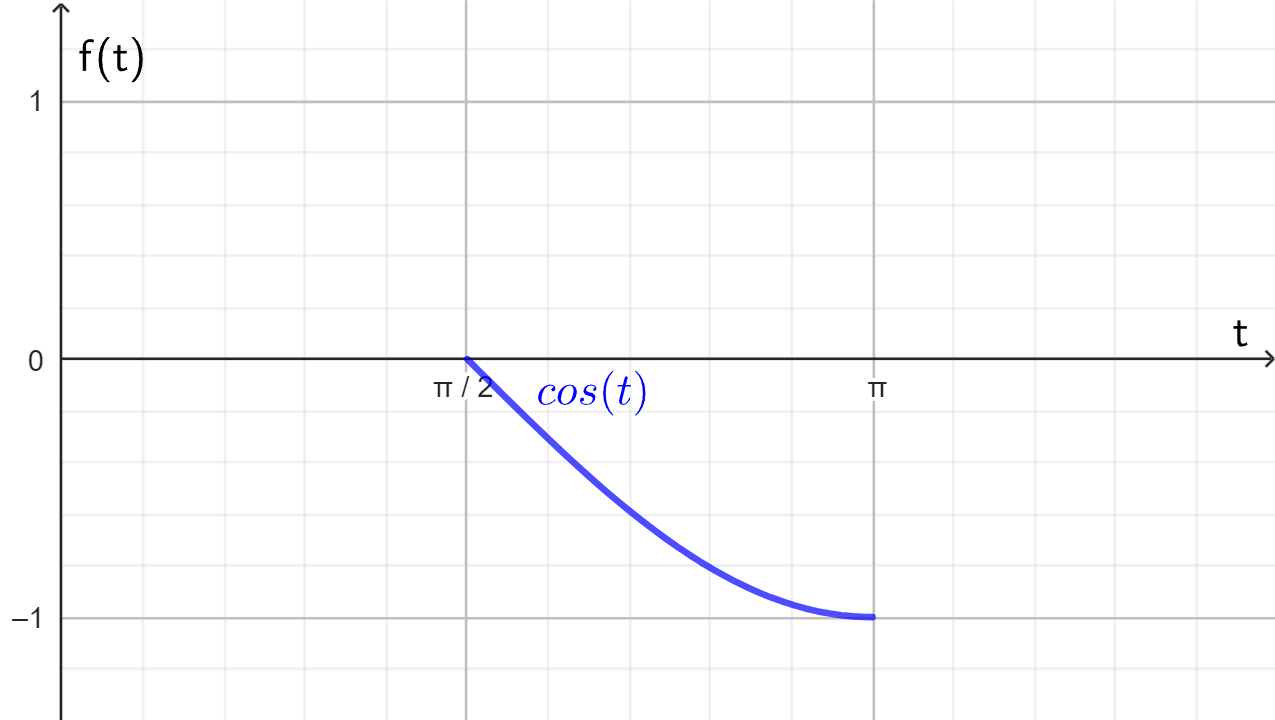
\includegraphics[width=0.45\textwidth]{VII.png}
\end{figure}
\addsubsection{Тригонометрический ряд Фурье}
Тригонометрический ряд Фурье выглядит так:
$$\frac{a_0}{2} + \sum\limits_{n = 1}^{\infty}a_n\cos{n\omega t} + b_n\sin{n\omega t}$$
Здесь $\omega = \nicefrac{2\pi}{T}$, $T$ --- длина промежутка, на котором задана исходная функция $f(t)$. Итак, $T = \pi - \nicefrac{\pi}{2} = \nicefrac{\pi}{2}$, $\omega = 4$. А коэффициенты $a_n$ и $b_n$ вычисляются так:
$$\begin{aligned}
    a_n &= \frac{2}{T}\int\limits^b_af(t)\cos{n\omega t}\,dt = \frac{4}{\pi}\int\limits^{\pi}_{\nicefrac{\pi}{2}}\cos{t}\,\cos{4nt}\,dt,&n = 0,\,1,\,2,\,\dots \\
    b_n &= \frac{2}{T}\int\limits^b_af(t)\sin{n\omega t}\,dt= \frac{4}{\pi}\int\limits^{\pi}_{\nicefrac{\pi}{2}}\cos{t}\,\sin{4nt}\,dt,&n = 1,\,2,\,3,\,\dots
\end{aligned}$$
Найдём $a_0$, $a_n$ и $b_n$:
$$a_0 = \frac{4}{\pi}\int\limits^{\pi}_{\nicefrac{\pi}{2}}\cos{t}\,dt = \frac{4}{\pi}(\sin{t})\at^\pi_{\nicefrac{\pi}{2}} \shiftright{4mm}{2mm}{=} \frac{4}{\pi}(\sin{\pi}-\sin{\nicefrac{\pi}{2}}) = - \frac{4}{\pi}$$
$$a_n = \frac{4}{\pi}\int\limits^{\pi}_{\nicefrac{\pi}{2}}\cos{t}\,\cos{4nt}\,dt = \frac{4}{\pi}\left( \frac{\sin{(4n+1)t}}{2(4n+1)} + \frac{\sin{(4n-1)t}}{2(4n-1)} \right)\at^\pi_{\nicefrac{\pi}{2}} \shiftright{4mm}{2mm}{=} \frac{4}{\pi(16n^2-1)}$$
$$b_n = \frac{4}{\pi}\int\limits^{\pi}_{\nicefrac{\pi}{2}}\cos{t}\,\sin{4nt}\,dt = \frac{4}{\pi}\left( \frac{\cos{(4n+1)t}}{2(4n+1)} + \frac{\cos{(4n-1)t}}{2(4n-1)} \right)\at^\pi_{\nicefrac{\pi}{2}} \shiftright{4mm}{2mm}{=} \frac{n}{\pi\left( n^2-\frac{1}{16} \right)}$$
$$\msquared{\displaystyle f(t) = -\frac{2}{\pi} + \sum\limits_{n=1}^{\infty}\frac{4\cos{4nt}}{\pi(16n^2-1)}+\frac{n\sin{4nt}}{\pi\left( n^2-\frac{1}{16} \right)},\ \ t \in \left( \frac{\pi}{2}, \pi\right)}$$\clearpage\noindent
И вот как выглядит график ряда с технически доступной точностью --- он выделен серым на фоне функции $f(t) = \cos{t}$:
\begin{figure}[H]
    \centering 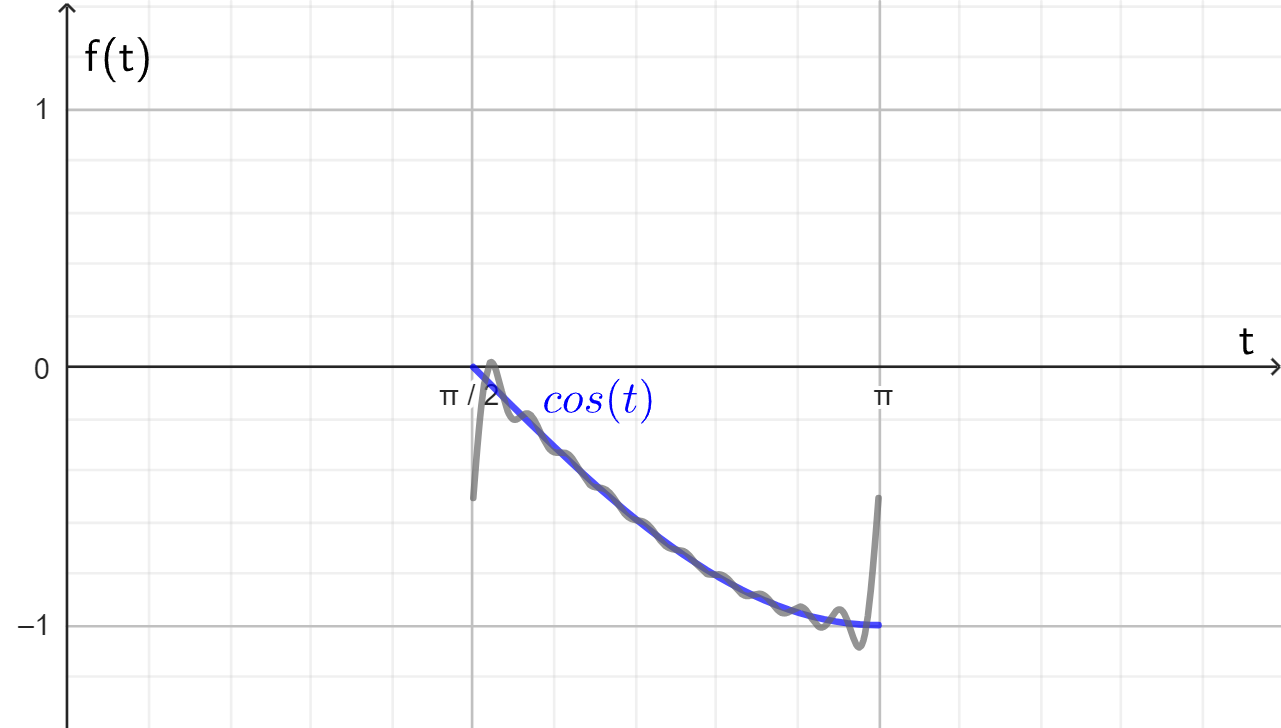
\includegraphics[width=0.45\textwidth]{VII (тригонометрический).png}
\end{figure}
\addsubsection{Ряд Фурье по синусам}
Поскольку ряд Фурье по синусам применим только к нечётным функциям, продолжим функцию нечётным образом через $-\cos{t}$ на промежутке $[-\pi, -\nicefrac{\pi}{2}]$. Обозначим полученную функцию как $\tilde{f}(t)$ и так будет выглядит ряд Фурье по синусам в общем виде:
$$\tilde{f}(t) \doteq \sum\limits_{n=1}^\infty \tilde{b}_n\sin{n\omega t}$$ График функции будет представлен позже вместе с графиком ряда Фурье.\\[2mm]
Обозначим константы: $T = \pi$, $\omega = 2$ и остаётся только коэффициент $\tilde{b}_n$:
$$\tilde{b}_n = \frac{4}{T}\int\limits_{0}^{\nicefrac{T}{2}}f(t)\sin{n\omega t}\,dt,\ n = 1,\,2,\,\dots$$
Вычислим этот коэффициент:
$$\tilde{b}_n = \frac{4}{\pi}\int\limits_0^{\nicefrac{\pi}{2}}\cos{t}\sin{2nt}\,dt -  = \frac{4}{\pi}\left( \frac{\cos{(2n+1)t}}{2(2n+1)} + \frac{\cos{(2n-1)t}}{2(2n-1)} \right)\at^{\nicefrac{\pi}{2}}_0  \shiftright{4mm}{2mm}{=} \frac{8n}{\pi(4n^2-1)}$$
Получаем такой ряд по синусам для заданной нами функции:
$$\msquared{\displaystyle \tilde{f}(t) = \sum\limits_{n=1}^\infty \frac{8n\sin{2nt}}{\pi(4n^2-1)},\ \ t \in \left(-\pi, -\frac{\pi}{2}\right) \cup \left( \frac{\pi}{2}, \pi\right)}$$
И так выглядит график ряда вместе с графиком функции $\tilde{f}(t)$:
\begin{figure}[H]
    \centering 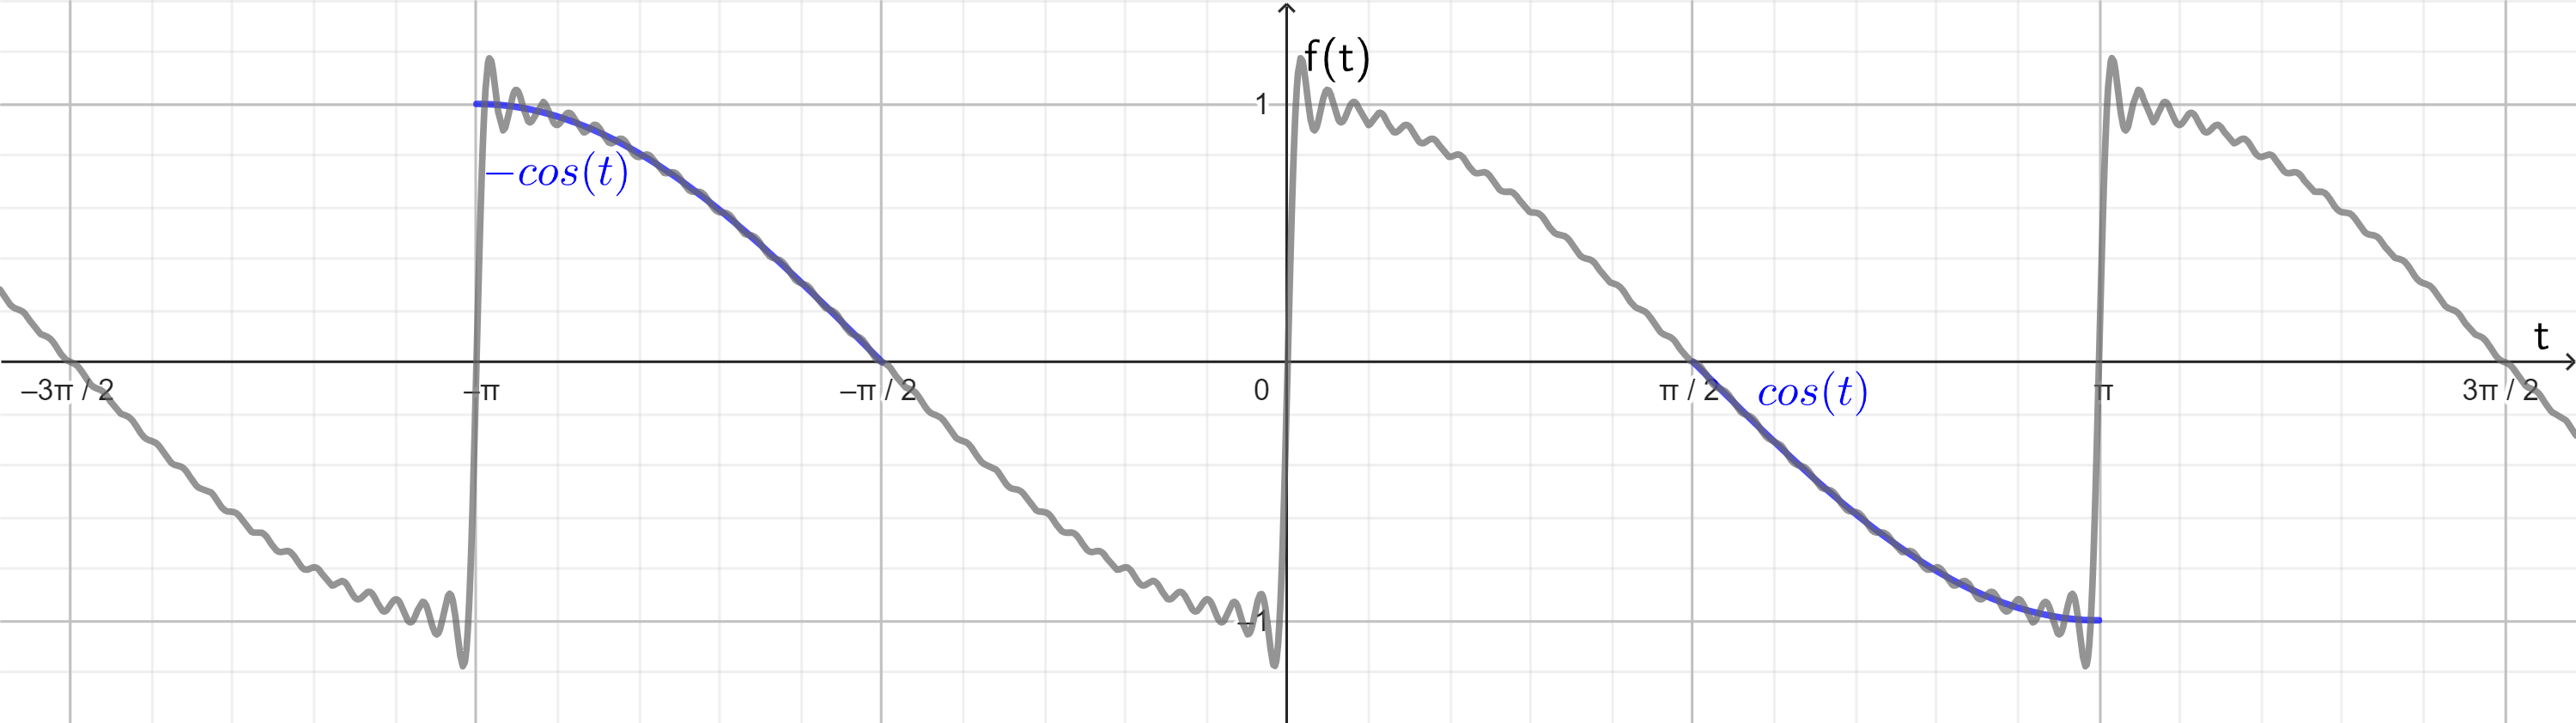
\includegraphics[width=0.9\textwidth]{VII (по синусам).png}
\end{figure}
\addsubsection{Ряд Фурье по косинусам}
Этот ряд, наоборот, существует только для чётных функций, поэтому продолжаем исходную функцию на промежутке $[-\pi, -\nicefrac{\pi}{2}]$. Вот как выглядит ряд Фурье по косинусам в общем виде:
$$f(t) = \frac{a_0}{2} + \sum\limits_{n=1}^{\infty}a_n\cos{n\omega t}\text{,\quad где } a_n = \frac{4}{T}\int\limits_{0}^{\nicefrac{T}{2}}f(t)\cos{n\omega t}\,dt,\ n = 0,\,1,\,2,\,\dots$$
Вновь обозначим константы $T = \pi$, $\omega = 2$, а $a_0$ мы сейчас найдём вместе с $a_n$:
$$a_0 = \frac{4}{\pi}\int\limits_{0}^{\nicefrac{\pi}{2}}\cos{t}\,dt = \frac{4}{\pi}\left( \sin{t} \right)\at^{\nicefrac{\pi}{2}}_0 = \frac{4}{\pi}$$
$$a_n = \frac{4}{\pi}\int\limits_{0}^{\nicefrac{\pi}{2}}\cos{t}\cos{2nt}\,dt = \frac{4}{\pi}\left( \frac{\sin{(2n+1)t}}{2(2n+1)} + \frac{\sin{(2n-1)t}}{2(2n-1)} \right)\at^{\nicefrac{\pi}{2}}_0 \shiftright{4mm}{2mm}{=} \frac{4\cdot(-1)^n}{\pi(4n^2-1)}$$
Получаем такой ряд по косинусам для заданной функции:
$$\msquared{\displaystyle f(t) = \frac{2}{\pi} + \sum\limits_{n=1}^{\infty}\frac{4\cdot(-1)^n\cos{2nt}}{\pi(4n^2-1)},\ \ t \in \left(-\pi, -\frac{\pi}{2}\right) \cup \left( \frac{\pi}{2}, \pi\right)}$$
И так выглядит график ряда вместе с графиком функции $\tilde{f}(t)$:
\begin{figure}[H]
    \centering 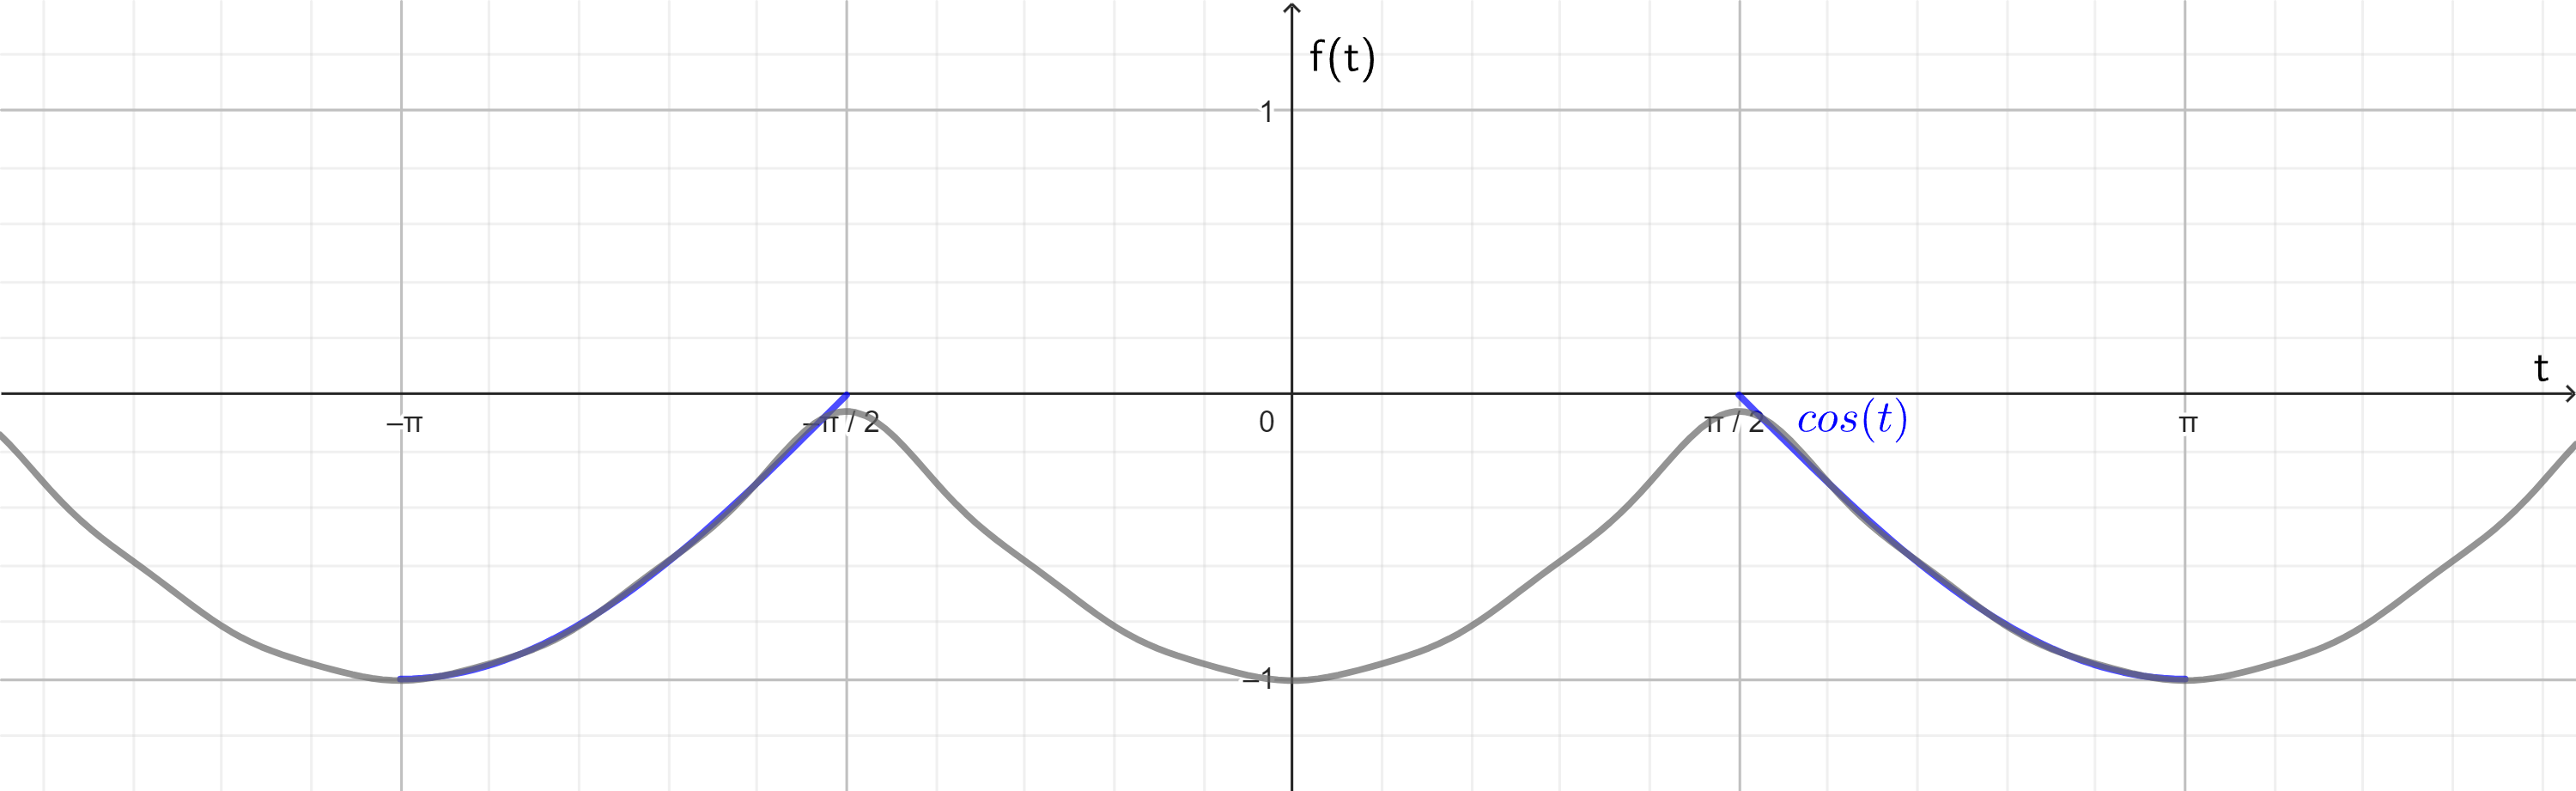
\includegraphics[width=0.9\textwidth]{VII (по косинусам).png}
\end{figure}
\addsubsection{Ряд Фурье в комплексной форме}
Ряд Фурье в комплексной форме имеет вид: $$f(t) = c_0 + \sum_{n=-\infty}^{\infty}c_ne^{i\omega nt}\text{,\quad где } c_n = T^{-1}\int\limits_{a}^{b}f(t)e^{-i\omega nt}\,dt$$
Вновь обозначим константы $T = \nicefrac{\pi}{2}$, $\omega = 4$ и найдём $c_0$ и $c_n$:
$$c_0 = \frac{2}{\pi}\int\limits_{\nicefrac{\pi}{2}}^{\pi}\cos{t}\,dt = -\frac{2}{\pi}$$
$$c_n = \frac{2}{\pi}\int\limits_{\nicefrac{\pi}{2}}^{\pi}\cos{t}e^{-4int}\,dt = \frac{2}{\pi}\cdot\frac{\sin{t}-4in\cos{t}}{(16n^2 - 1)e^{4int}}\at_{\nicefrac{\pi}{2}}^{\pi} \shiftright{4mm}{2mm}{=} \frac{2e^{2i\pi n} - 8in}{\pi(16n^2-1)e^{4i\pi n}}$$
Получаем следующий ряд в комплексной форме для функции $f(t)$:
$$\msquared{\displaystyle f(t) = -\frac{2}{\pi} + \sum_{n=-\infty,\ n\ne\nicefrac{1}{4}}^{\infty} \frac{2e^{2i\pi n} - 8in}{\pi(16n^2-1)e^{4i\pi n}}e^{4int},\ \ t \in \left( \frac{\pi}{2}, \pi\right)}$$
\addsection{Задание №8}
Функция задана на всей области через два промежутка:
$$f(t) = \left\{ \begin{aligned}
    &\sin{2t},\ &t \in [-\pi, \pi] \\
    &0,\ &t \notin [-\pi, \pi]
\end{aligned} \right.$$
Прямое преобразование Фурье в комплексной форме для этой задачи выглядит так:
$$F(\omega) = (2\pi)^{-\nicefrac{1}{2}}\int\limits_a^b f(t)e^{i\omega t}\,dt$$
Подставим $\sin{2t}$ вместо $f(t)$ и $a=-\pi$, $b=\pi$:
$$F(\omega) = \frac{1}{\sqrt{2\pi}}\int\limits_{-\pi}^{\pi}\sin{2t}e^{i\omega t} = \frac{1}{\sqrt{2\pi}}\frac{e^{i\omega t}(2\cos{2t}-i\omega\sin{2t})}{\omega^2-4}\at^\pi_{-\pi} = \msquared{\displaystyle \frac{2(e^{2i\pi \omega} - 1)}{\sqrt{2\pi}(\omega^2-4)e^{i\pi\omega}}}$$
\end{document}